%Original Format

% Dieser Text ist urheberrechtlich gesch�tzt
% Er stellt einen Auszug eines von mir erstellten Referates dar
% und darf nicht gewerblich genutzt werden
% die private bzw. Studiums bezogen Nutzung ist frei
% Nov. 2007
% Autor: Sascha Frank 
% Universit�t Freiburg 
% www.informatik.uni-freiburg.de/~frank/

%Vortrag:

% Aug 2018
% Autor: Dinah Tecle 
% Universität Siegen 

\PassOptionsToPackage{unicode}{hyperref}  
\documentclass{beamer}
\newcommand{\gauss}[1]{\lfloor #1 \rfloor}
\newcommand{\menge}[2]{\left\{#1\:\middle|\:#2\right\}}

\usetheme{Warsaw}
%\usepackage{hyperref}
\usepackage{bookmark}
\usepackage[ngerman]{babel}
\usepackage[utf8]{inputenc}
\beamersetuncovermixins{\opaqueness<1>{25}}{\opaqueness<2->{15}}

\begin{document}
\title{Analyse zur Fleissner-Schablone}  
\author{Dinah Tecle}
\date{\today} 

\setbeamertemplate{footline}[page number]
\begin{frame}
\titlepage
\end{frame} 

\begin{frame}
\frametitle{Inhaltsverzeichnis}\tableofcontents
\end{frame} 


\section{Fleissner-Schablone} 
\begin{frame}
\begin{center}
\textbf{\huge Fleissner-Schablone}
\end{center}
\end{frame}

\subsection{Hintergrund}
\begin{frame}
\frametitle{Was ist die Fleissner-Schablone?} 
\begin{itemize}
\item Kategorie: Transpositionsverfahren
\item Entwickelt 1881 von Eduard Fleissner von Wostrowitz
\item Jules Verne griff das Verfahren 1885 in seinem Roman \glqq Mathias Sandorf\grqq{} auf.
\item Die Schablone wurde im ersten Weltkrieg auf deutscher Seite genutzt.
\item Das Verfahren ist mittlerweile veraltet und heute nicht mehr sicher.
\end{itemize}
\end{frame}


\begin{frame} 
\frametitle{Was ist die Fleissner-Schablone?} 
Beispiel einer $12 \times 12$-Schablone
\begin{figure}
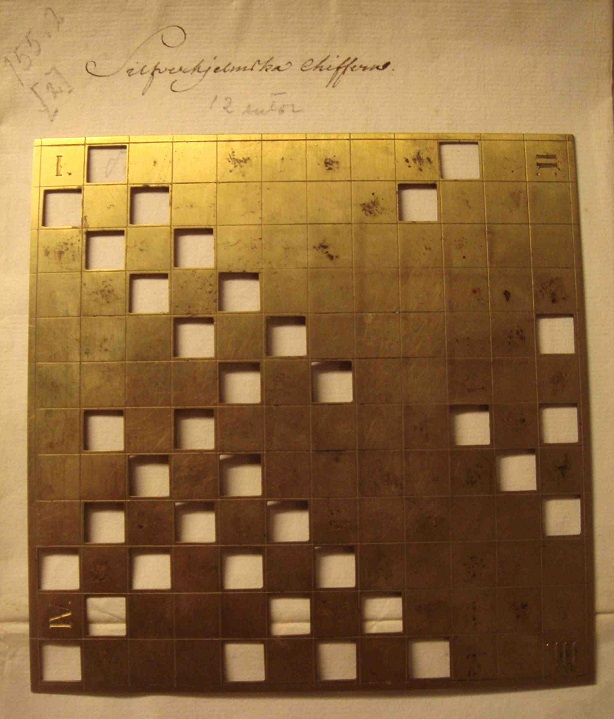
\includegraphics[scale=0.2]{Fleissner-Grille.jpg} 
\caption{\footnotesize Quelle: http://scienceblogs.de/klausis-krypto-kolumne/2017/01/13/fleissner-challenge-can-this-cryptogram-be-broken/}
\end{figure}
\end{frame}

\subsection{Verfahren}
\begin{frame} 
\frametitle{Wie erstellt man eine Fleissner-Schablone?} 
\begin{itemize}
\item Eine quadratische Schablone der Seitenlänge $n$, die in $n^2$ kleinere Quadrate
unterteilt wird%\pause
\item Nach einem (selbst-)bestimmten Muster werden einige kleinere Quadrate ausgeschnitten%\pause
\item Der Entwurf des Musters ist dabei Restriktionen ausgesetzt, da die Schablone bei ihrer Anwendung drei mal gedreht wird, und dabei keine Buchstaben übereinander geschrieben werden dürfen
\end{itemize}
\end{frame}

\begin{frame}
\frametitle{Wie erstellt man eine Fleissner-Schablone?} 
\vspace{0.2cm}
$\Rightarrow$ Beginnend mit dem Index $0$ und der Bezeichnung (Spalte, Zeile)\\ für eine Koordinate, wobei $(0,0)$ das Feld oben links und $(3,3)$ das Feld unten rechts bezeichnet, fallen beispielsweise bei der Wahl von $(x,y)=(0,1)$ für $n=4$ die drei Koordinaten $(n-1-y,x)=(2,0)$, $(n-1-x,n-1-y)=(3,2)$ und $(y,n-1-x)=(1,3)$ weg.%\pause

\begin{columns}
\begin{column}{5cm}
Ausgewählte Koordinate: Kreis\\
Blockierte Koordinaten: Grau
\vspace{2cm}
\end{column}
\begin{column}{4.5cm}
\begin{figure}
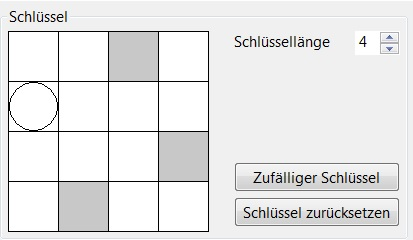
\includegraphics[scale=0.5]{firstHole.jpg}
\caption{\small Quelle: JCrypTool}
\end{figure}
\vspace{2cm}
\end{column}
\end{columns}
\end{frame}

\begin{frame}
\frametitle{Wie erstellt man eine Fleissner-Schablone?} 
\begin{itemize}
\item Ein fertiges Muster kann als Abfolge von Koordinaten der ausgeschnittenen Quadrate der Form (Spalte,Zeile,Spalte,Zeile,...) beschrieben werden%\pause
\vspace{0.3cm}

\textbf{Beispiel:} Beginnend mit dem Index $0$\\
\hspace{1cm}
\begin{columns}
\begin{column}{4cm}
{\small
Muster $(\underbrace{0,1}_{\text{1. Koord.}},\underbrace{2,1}_{\text{2. Koord.}},\underbrace{0,3}_{\text{3. Koord.}},\underbrace{2,3}_{\text{4. Koord.}})$ }
\vspace{2cm}
\end{column}

\begin{column}{4.5cm}
\begin{figure}
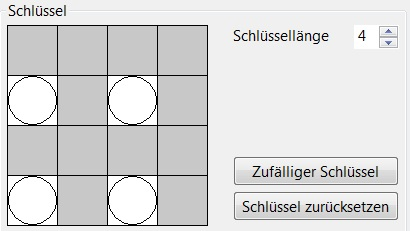
\includegraphics[scale=0.5]{Schablone4mal4.jpg}
\caption{\footnotesize Quelle: JCrypTool}
\end{figure}
\vspace{0.5cm}
\end{column}
\end{columns}
\end{itemize}
\end{frame}

\begin{frame}
\frametitle{Wie wendet man die Schablone an?}
\begin{itemize}
\item Die fertige Schablone wird auf ein Blatt gelegt und ausgeschnittene Quadrate von links nach rechts und von oben nach unten mit Klartextbuchstaben ausgefüllt.%\pause
\item Schablone wird um $90^\circ$ gedreht.%\pause
\item Wiederholung dieses Vorgangs, bis die Schablone in allen Rotationspositionen ausgefüllt wurde.
\end{itemize}
\end{frame}

\begin{frame} 
\frametitle{Eine Verschlüsselungsrunde} 
Gegeben ist der Klartext \glqq WIKIPEDIA DIE FREIE ONLINE ENZYKLOPAEDIE\grqq{}. Leerzeichen zwischen Worten werden ignoriert. Hier ist $n=6$.
\begin{figure}
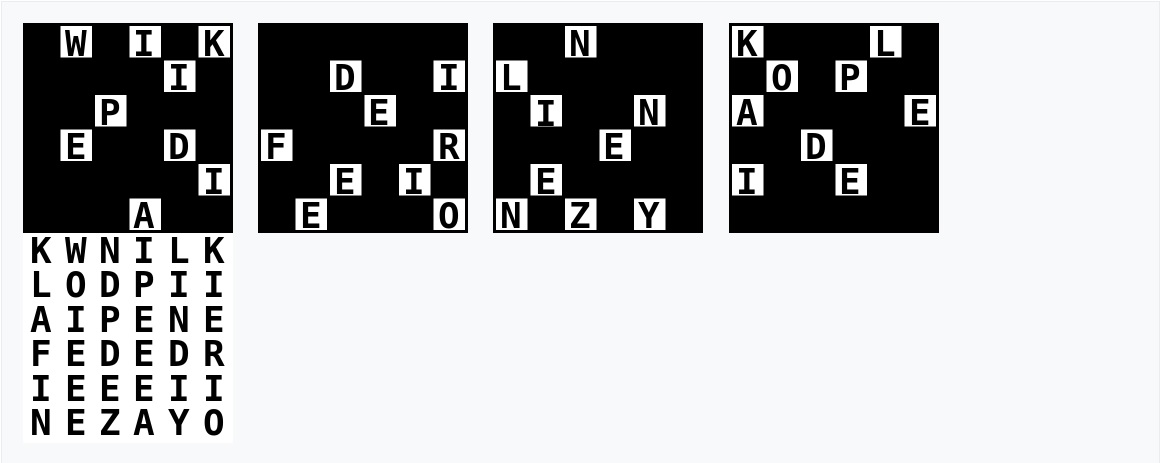
\includegraphics[scale=0.4]{WikiVerschluesselung.jpg}
\caption{Quelle: \url{https://de.wikipedia.org/wiki/Flei\%C3\%9Fnersche_Schablone}}
\end{figure}
\end{frame}

\section{Analyse} 
\begin{frame}
\begin{center}
\textbf{\huge Analyse}
\end{center}
\end{frame}

\subsection{Grundlagen}
\begin{frame}\frametitle{Idee der Analyse}
\begin{itemize}
\item Fleissner-Schablone ist eine Transpositionschiffre \\
$\Rightarrow$ Die Häufigkeit der Buchstaben bleibt unverändert.%\pause
\item Jede Sprache besitzt häufige und weniger häufige Buchstabenkombinationen%\pause
\item Buchstabenkombinationen verschiedener Längen $N$ werden als \glqq $N$-Gramme\grqq{} bezeichnet %\pause
\item $N$-Gramme besitzen der Sprache entsprechende Auftrittswahrscheinlichkeiten%\pause
\item Je mehr $N$-Gramme mit hohen Auftrittswahrscheinlichkeiten im vorliegenden Text auftauchen, desto eher liegt ein korrekter Text in der jeweiligen Sprache vor.%\pause
\item In einem Analyseverfahren wird der \glqq Wert\grqq{} des Textes durch eine Kostenfunktion bestimmt, der zuvor $N$-Gramme mit ($\log$-)Wahrscheinlichkeiten übergeben wurden.
\end{itemize}
\end{frame}

\begin{frame}\frametitle{Ansatz für die Analyse}
\begin{itemize}
\item Die Anzahl der möglichen Schablonen hängt von der Schablonengröße ab und bestimmt die Analysemethode%\pause
\item Ist die Anzahl der möglichen Schablone \glqq klein genug\grqq{}, wählt man die \glqq Brute-Force\grqq-Methode. Dabei werden alle möglichen Schablonen (Schlüssel) durchlaufen und für jeden Durchlauf die Kostenfunktion berechnet%\pause
\item Bei ansteigender Anzahl der Möglichkeiten bietet sich \glqq Hill-Climbing\grqq{} an
\end{itemize}
\end{frame}

\subsection{Aufbau}
\begin{frame}\frametitle{Hill-Climbing (Bergsteigeralgorithmus)}
\begin{itemize}
\item Heuristisches Optimierungsverfahren %\pause
\item Verschiedene Startpunkte, so dass verschiedene Extrempunkte erreicht werden können%\pause
\item Schritt-für-Schritt Verbesserungen%\pause
\item Abbruch, nachdem über längere Zeit keine Verbesserung mehr erzielt wurde\\
$\Rightarrow$ Bei \glqq ausreichend\grqq{} vielen Neustarts wird der richtige Schlüssel mit hoher Wahrscheinlichkeit gefunden.
\end{itemize}
\end{frame}

\begin{frame}\frametitle{Parameter}
\begin{itemize}
\item Schlüsselmenge (Menge unterscheidbarer, quadratischer Schablonen) $\Omega$, wobei $|\Omega|\hat{=}$ Anzahl der Elemente von $\Omega$,%\pause
\item Schlüssel (Schablone) $S\in\Omega$,%\pause
\item Länge $n \in \mathbb{N}_{\geqslant 2}$ der Schablone,%\pause
\item Anzahl Löcher $h$ (wie \glqq holes\grqq)
\end{itemize}
\end{frame}

\begin{frame}\frametitle{Berechnung der Parameter}
Bedingungen für die Modellierung:
\begin{enumerate}
\item Für gerade $n$ soll nach Anwendung der Schablone \underline{kein} Feld frei bleiben, für ungerade $n$ soll das mittlere Feld frei bleiben.%\pause
\item Mit der Wahl eines Felds dürfen die drei Felder, die durch die Drehung der Schablone angenommen werden, nicht mehr zur Wahl stehen.%\pause
\end{enumerate}

Wegen (1) stehen $n^2$ Felder für gerade $n$ und $n^2-1$ Felder für ungerade $n$ für die Wahl von $h$ zur Verfügung. Wegen (2) muss aber noch durch $4$ geteilt werden. %\pause
\[
\Rightarrow h=\begin{cases}
\frac{n^2}{4},&\text{ falls }n \text{ gerade }\\
\frac{n^2-1}{4}, & \text{ falls } n\text{ ungerade }
\end{cases}
\]
\end{frame}

\begin{frame}\frametitle{Berechnung der Parameter}
{\small Auswahl der Löcher kann wie Urnenmodell aufgebaut werden:%\pause 
\vspace*{0.2cm}

Es wird aus $h$ Urnen jeweils eine aus vier möglichen Kugeln gezogen (hier: Jede Urne enthält die vier zusammengehörigen Felder, die durch Drehungen der Schablone angenommen werden).%\pause 
\\
Die Menge der Schablonen kann dann als\\
\begin{center}
$\Omega=\menge{\{a_{i,1},\dotsc ,a_{i,h}\}}{i\in\{1,\dotsc ,4\}}$
\end{center}
beschrieben werden.%\pause 
\\
Ohne Beachtung der Reihenfolge, da jede Permutation der Elemente eines $S=\{a_{i,1},\dotsc ,a_{i,h}\} \in\Omega$ die gleiche Schablone erzeugt.%\pause 
\\
Die Anzahl\footnote{\tiny siehe \hyperlink{anhang}{Anhang}}
%[sec:Modell]
  $|\Omega|$ berechnet sich dann zu
\[
|\Omega|=\binom{h}{h}\cdot 4^h=4^h
\]}
\end{frame}


\begin{frame}\frametitle{Anzahl der Möglichkeiten für $n\in\{2,\dotsc ,12\}$}

{\footnotesize
\begin{tabular}{c|c|c|c|c}
$n$ & $h$ & $|\Omega|$ & Verfahren  & Laufzeit\footnote{\tiny Durchschnitt nach 10 Durchläufen (Durchlauf $\hat{=}$ Neustart des Analyseprogramms), Restarts (für Hill-Climbing): 50, Textlänge: 963 Zeichen (ohne Leerzeichen), Sprache: Deutsch} (in ms)\\\hline
2 & 1 & 4 & Brute-Force & 102,4 {\tiny(Erfolg 10/10)}\\
3 & 2 & 16 & Brute-Force & 302,7 {\tiny(Erfolg 10/10)}\\
4 & 4 & 256 & Brute-Force & 4411,2 {\tiny(Erfolg 10/10)}\\
5 & 6 & 4.096 & Hill-Climbing &1946,9 {\tiny(Erfolg 10/10)}\\	
6 & 9 & 262.144 & Hill-Climbing & 2522,2 {\tiny(Erfolg 10/10)}\\
7 & 12 & 16.777.216 & Hill-Climbing & 3236 {\tiny(Erfolg 9/10)}\\
8 & 16 & 4.294.967.296 & Hill-Climbing & 4216,2 {\tiny(Erfolg 9/10)}\\
9 & 20 & 1.099.511.627.776 & Hill-Climbing & 5299,9 {\tiny(Erfolg 7/10)}\\
10 & 25 & 1.125.899.906.842.624 & Hill-Climbing & 6544,9 {\tiny(Erfolg 7/10)}\\
11 & 30 & 1.152.921.504.606.846.976 & Hill-Climbing & 7987,3 {\tiny(Erfolg 2/10)}\\
12 & 36 & 4.722.366.482.869.645.213.696 & Hill-Climbing & 9696,5 {\tiny(Erfolg 4/10)}
\end{tabular}}
\end{frame}


\section{Anwendung} 
\begin{frame}
\begin{center}
\textbf{\huge Anwendung}
\end{center}
\end{frame}

\subsection{\texorpdfstring{$4 \times 4$-Schablone}{4 × 4-Schablone}}
\begin{frame}
\frametitle{$4 \times 4$-Schablone}
\begin{columns}
\begin{column}{4cm}
\vspace{1cm}
\begin{itemize}
\item $4 \times 4$-Schablone
\item Schablone $S=(0,1,2,1,0,3,2,3)$
\item Analysemethode: Brute-Force ($|\Omega|=4^4= 256$)
\end{itemize}
\vspace{3cm} 
\end{column}
\hspace{1cm}
\begin{column}{5cm}
\begin{figure}
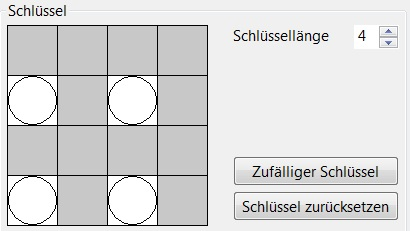
\includegraphics[scale=0.6]{Schablone4mal4.jpg}
\caption{Quelle: JCrypTool}
\end{figure}
\vspace{1cm}
\end{column}
\end{columns}
\end{frame}



\begin{frame}
\frametitle{Analyse zur $4 \times 4$-Schablone}
\begin{figure}
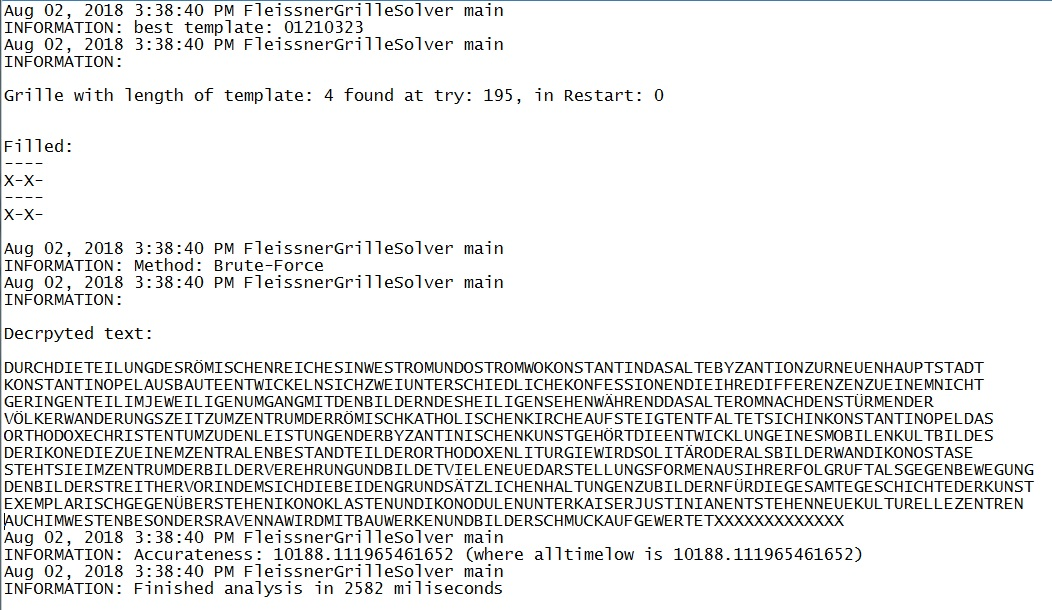
\includegraphics[scale=0.45]{Ausgabe4Mal4.jpg} 
\caption{Ausgabe nach Brute-Force}
\end{figure}
\end{frame}

\subsection{\texorpdfstring{$5 \times 5$-Schablone}{5 × 5-Schablone}} 
\begin{frame}
\frametitle{$5 \times 5$-Schablone}
\begin{columns}
\begin{column}{4cm}
\vspace{1cm}
\begin{itemize}
\item $5 \times 5$-Schablone
\item Schablone $S=(2,0,0,1,3,1,1,2,0,3,0,4)$
\item Analysemethode: Hill-Climbing \\($|\Omega|=4^6= 4096$)
\end{itemize}
\vspace{3cm} 
\end{column}
\hspace{0.5cm}
\begin{column}{5cm}
\begin{figure}
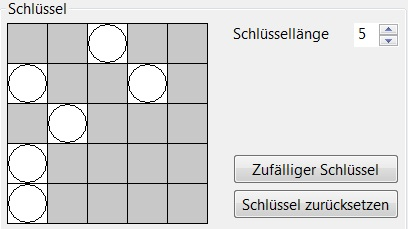
\includegraphics[scale=0.65]{Schablone5mal5.jpg}
\caption{Quelle: JCrypTool}
\end{figure}
\vspace{1cm}
\end{column}
\end{columns}
\end{frame}


\begin{frame}
\frametitle{Analyse zu $5 \times 5$-Schablone}
\begin{figure}
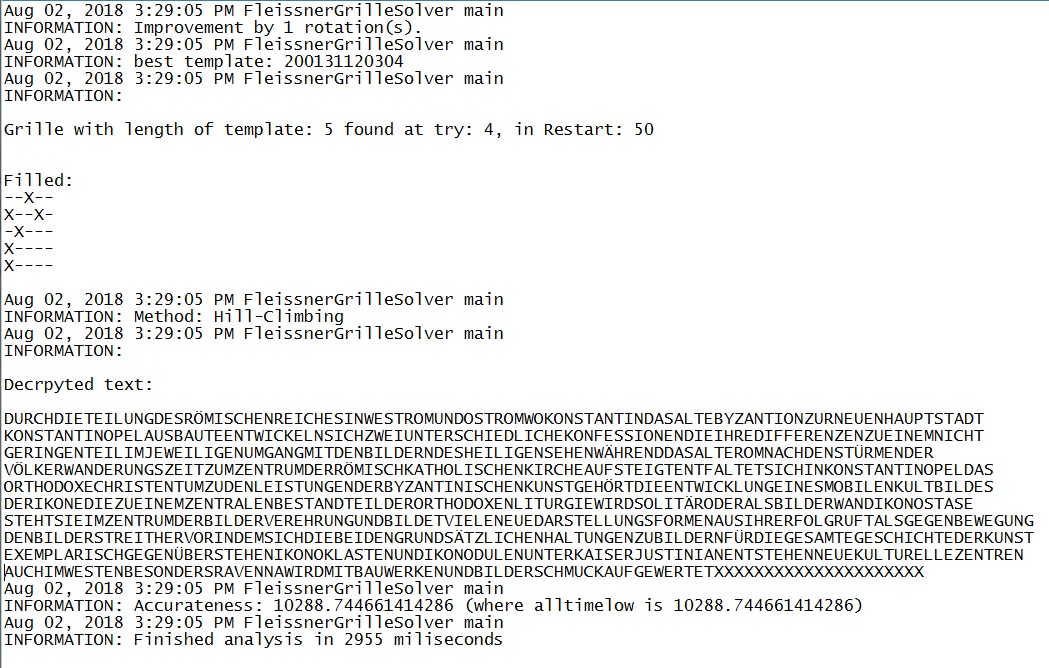
\includegraphics[scale=0.4]{Ausgabe5Mal5.jpg} 
\caption{Ausgabe nach Hill-Climbing}
\end{figure}
\end{frame}


\subsection{\texorpdfstring{$8 \times 8$-Schablone}{8 × 8-Schablone}} 
\begin{frame}
\frametitle{$8 \times 8$-Schablone}
\begin{columns}
\begin{column}{5cm}
\vspace{1cm}
\begin{itemize}
\item $8 \times 8$-Schablone
\item Schablone $S=(1,0,5,0,2,1,4,1,6,1,1,2,7,2,0,3,$\\$3,3,5,3,1,4,3,5,5,5,7,6,0,7,4,7)$
\item Analysemethode: Hill-Climbing \\($|\Omega|=4^{16}> 4$ Mrd.)
\end{itemize}
\vspace{3cm} 
\end{column}
\hspace{1cm}
\begin{column}{5cm}
\begin{figure}
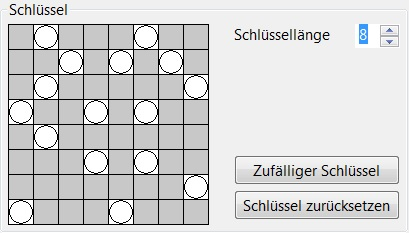
\includegraphics[scale=0.6]{Schablone8mal8.jpg}
\caption{Quelle: JCrypTool}
\end{figure}
\vspace{1cm}
\end{column}
\end{columns}
\end{frame}


\begin{frame}
\frametitle{Analyse zu $8 \times 8$-Schablone}
\begin{figure}
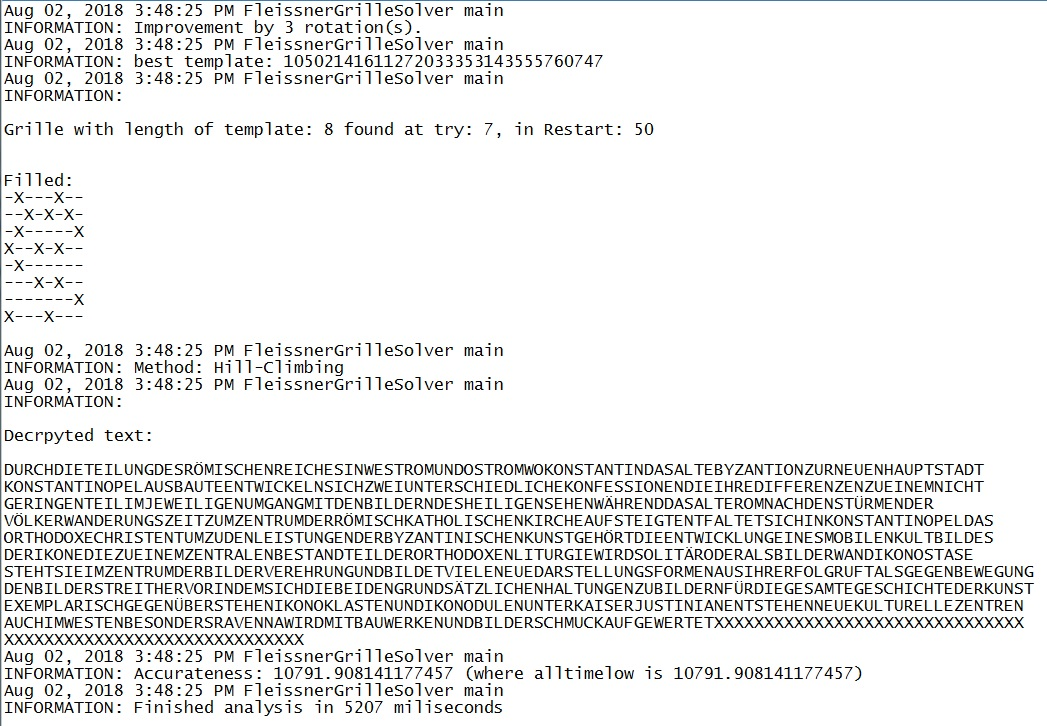
\includegraphics[scale=0.4]{Ausgabe8Mal8.jpg} 
\caption{Ausgabe nach Hill-Climbing}
\end{figure}
\end{frame}

\section{Anhang}\hypertarget{anhang}{}
%\label{anhang}
%\label{anhang}
% {Anhang}
%\label{sec:Modell}
%\phantomsection 
\begin{frame}
\begin{center}
\textbf{\huge Anhang: \\Mathematische Modellierung zum Aufbau der Fleißner-Schablone}
\end{center}
\end{frame}

\subsection{Mathematische Modellierung zum Aufbau der Fleißner-Schablone}
\begin{frame}
\frametitle{Anhang}
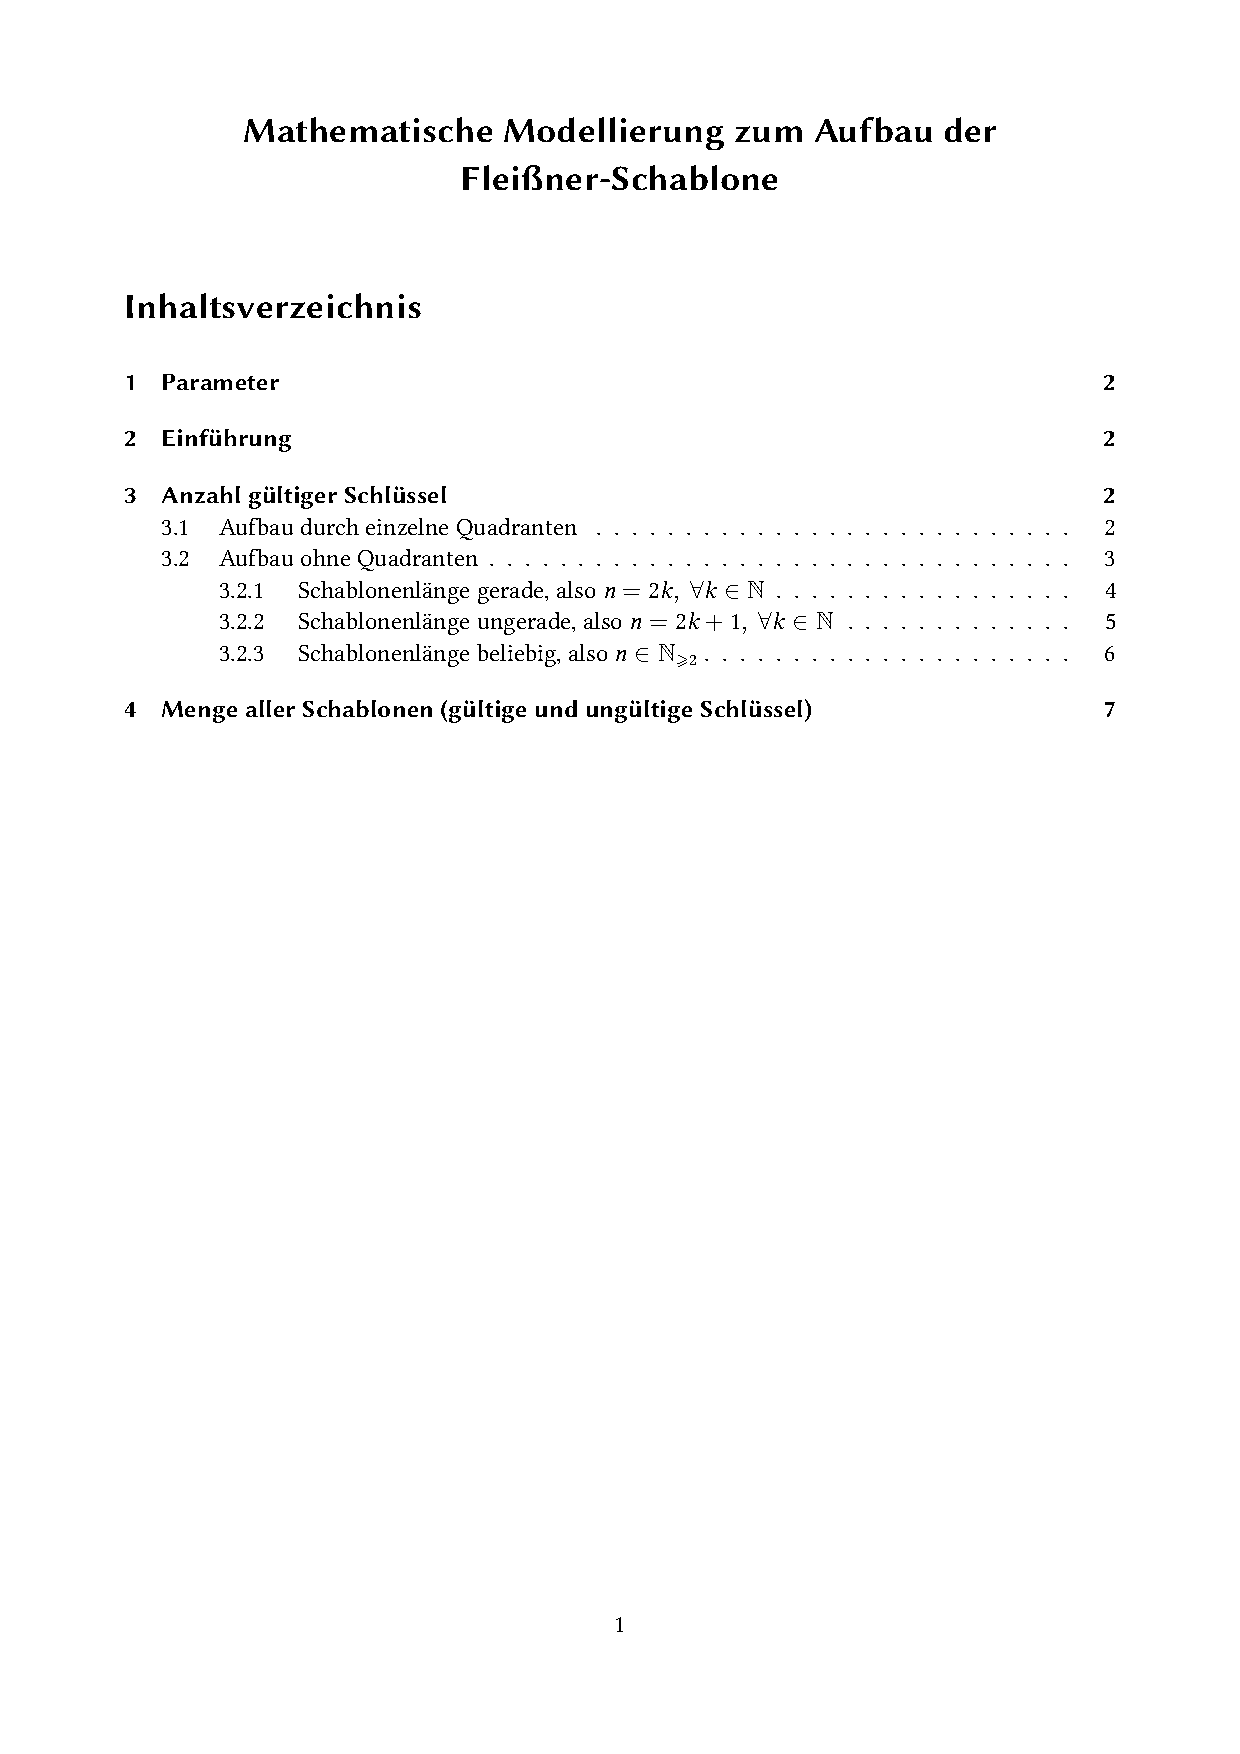
\includegraphics[page=1, scale=0.4]{mathModell2.pdf}
\end{frame}

\begin{frame}
%\frametitle{Anhang: Mathematische Modellierung zur Anzahl möglicher Schablonen}
\includegraphics[page=2, scale=0.25]{mathModell.pdf}
\includegraphics[page=3, scale=0.25]{mathModell.pdf}
\end{frame}

\begin{frame}
%\frametitle{Anhang: Mathematische Modellierung zur Anzahl möglicher Schablonen}
\includegraphics[page=4, scale=0.25]{mathModell.pdf}
\includegraphics[page=5, scale=0.25]{mathModell.pdf}
\end{frame}

\begin{frame}
%\frametitle{Stochastische Modellierung zur Anzahl möglicher Schablonen}
\includegraphics[page=6, scale=0.25]{mathModell.pdf}
\includegraphics[page=7, scale=0.25]{mathModell.pdf}
\end{frame}
\end{document}